\section{Differential Atmospheric Refraction}
\label{chap:DAR}

\def\hdrldar{{\em hdrl\_dar}}
\def\hdrlcat{{\em hdrl\_catalogue}}
\def\hdrlstrehl{{\em hdrl\_strehl}}



\subsection{Introduction}

The effects of atmospheric refraction can be readily seen in any spectrograph or IFU. Atmospheric refraction will displace a source, or its spectrum, 
by an amount that is dependent on the source wavelength and the angular distance of the source from the zenith.  
This effect is due to the stratified density structure of our atmosphere, and the displacement will be toward the zenith and will be largest for shorter wavelengths.
Because of this latter attribute, differential atmospheric refraction is not generally associated with infrared instruments. However, it can be 
readily seen in SINFONI data cubes observed with the largest wavelength coverage (H+K) and in the smallest pixel scales (25 mas). 
Here, the shift can be as large as 6 pixels from the beginning of the data cube to its end (see Figures \ref{fig:SINFONI_trace} and \ref{fig:SINFONI_image}).

This module uses an analytical approach to compute the expected differential refraction as a function of wavelength, zenith angle, and the refractive index of air
which, in turn, depends on temperature, pressure, and water vapour pressure.

The \hdrldar\ routines require the following inputs (all of which are, generally, available in the input data headers):
\begin{itemize}
\item the ambient atmospheric parameters: temperature, pressure, and humidity as contained in the environmental keyword headers:
TEL.AMBI.TEMP, TEL.AMBI.PRES.START/END, and TEL.AMBI.RHUM, respectively.
\item the instrument rotation angle on the sky
\item the parallactic angle of instrument
\item and, the world-coordinate system (WCS)
\end{itemize}


\subsection{Testing HDRL DAR}
\label{chap:testing_DAR}

The goal of this test series is to compare the actual source displacements, as measured in processed SINFONI
data cubes, with the displacements predicted by \hdrldar.

SINFONI standard stars were selected for this comparison as they tend to be bright, display some flux for the full
wavelength range covered, and are point sources.   The standard star data was selected from the ESO archive for the years 2014, 2015, and 2016.  
Furthermore, this data was selected to cover the $J$ and $H + K$-bands as they are most susceptible to 
atmospheric refraction; the former because it is the bluest filter, and the latter because it covers the 
largest span in wavelength. Data from all three SINFONI image scales was used. In order to test the full range 
of parameters relevant to atmospheric refraction, an effort was made to ensure that the data covered a 
significant range of instrument rotation angles, airmasses, air pressures, temperatures, and relative humidities
(see Table \ref{fig:SINFONI_data}).

\begin{table}[ht]
\caption{Parameter Ranges Covered by SINFONI Data}
\begin{center}
\begin{tabular}{ l c c }
{\bf SINFONI Cube Parameter}			& \multicolumn{2}{l}{{\bf Range of Parameters}}  \\
  								& {\bf Minimum}	& {\bf Maximum} \\
 instrumental rotation angle [degrees]	& -230			& 234.2	   \\				
 airmass [degrees] 					& 1.001			& 2.350	   \\
 air pressure [HPa]                 			& 739.5   			& 747.8     \\
 temperature [$^\circ$C]      			& 3.4				& 20.0       \\
  relative humidity [\%]             			& 3.0    			& 63.0 	   \\
\end{tabular}
\end{center}
\label{fig:SINFONI_data}
\end{table}

The standard star data was processed using the SINFONI pipeline version 3.0.0 running as a Reflex workflow.  All processing parameters were left
in their default values.   In total, 754 SINFONI data cube products were created in this processing.    

\subsection{Testing the \hdrldar\ Differential Atmospheric Refraction Routines with SINFONI Data}

\subsubsection{I.  Method and Qualitative Results}

For each SINFONI data cube, a source centroid for each cube plane (omitting the first and last 100 planes due to higher noise levels) was computed, in order to measure
the actual source shifts due to atmospheric refraction.  This is done using the source detection catalogue routines (\hdrlcat) adapted from CASU (Madsen, G.,   
HAWK-I Pipeline User Manual, February 19, 2016.  Issue 1.0.).
For each of the 754 data cubes analysed, plots were created mapping the measured source centroids ($X_c$ and $Y_c$) as a function of wavelength through the data cube.    
For each of these source traces, the shift values computed by the \hdrldar\ output tables were applied to the centroids to correct the
differential atmospheric refraction.  A typical example of such a trace is shown in Figure \ref{fig:SINFONI_trace}.
A comparison of the median-collapsed cube images before and after being corrected for atmospheric refraction (at an integer shift level) is shown in Figure \ref{fig:SINFONI_image}.
In both plots, a significant qualitative improvement is apparent.

\begin{figure}[H]
\centering \subfigure
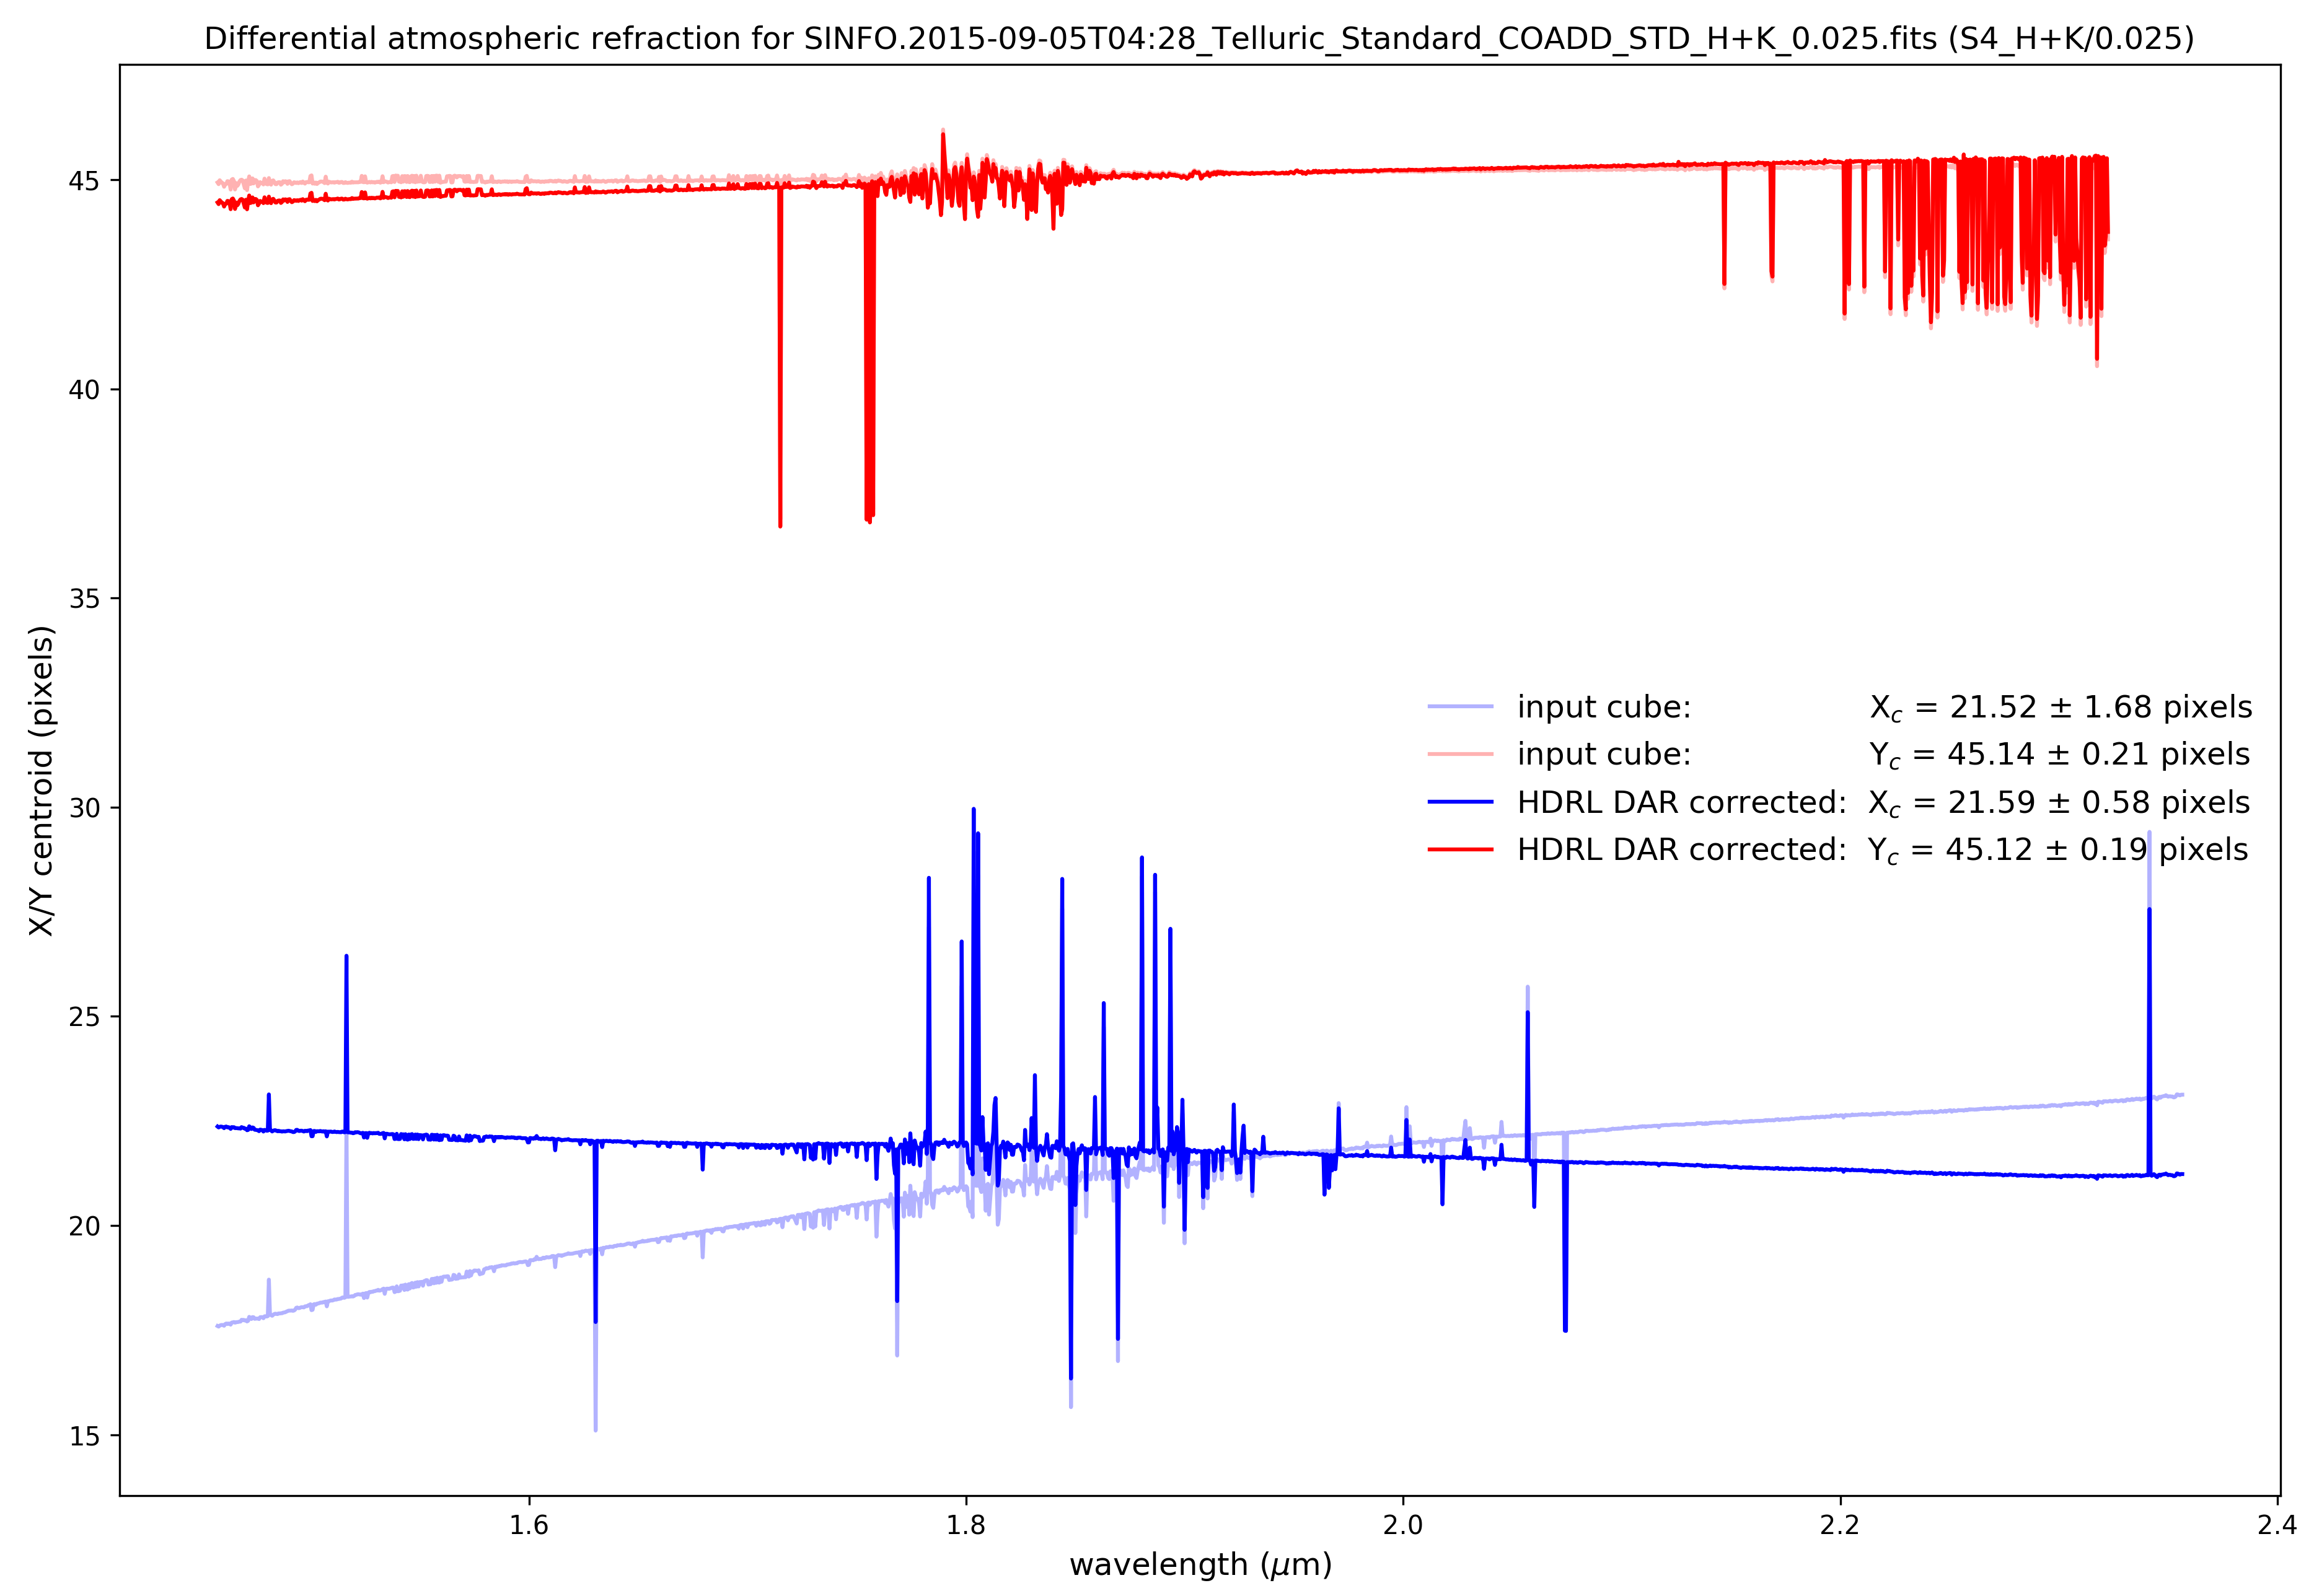
\includegraphics[width=16cm]{figures/SINFO_cube_centroid_corrected.png} 
\caption[]
	{\footnotesize  A line trace of the source centroid position as a function of wavelength for the SINFONI data cube {\tt SINFO.2015-09-05T04:28\_Telluric\_Standard\_COADD\_STD\_H+K\_0.025.fits}.  
	The source centroid is computed through the data cube using the catalogue source-detection module available in \hdrlcat.  
	The blue and red lines are the x-axis  (X$_c$) and y-axis centroids (Y$_c$), respectively.  The faded lines are the raw input data centroids, while the dark lines are the centroids 
	after being corrected for differential atmospheric refraction by \hdrldar.	   The raw data cube has a shift in the source
	centroid, over its full wavelength range, of $\Delta$X$_c$ = 6.9 and $\Delta$Y$_c$ = 0.2 pixels. 
	}
	\label{fig:SINFONI_trace}
\end{figure}

\begin{figure}[H]
\centering \subfigure
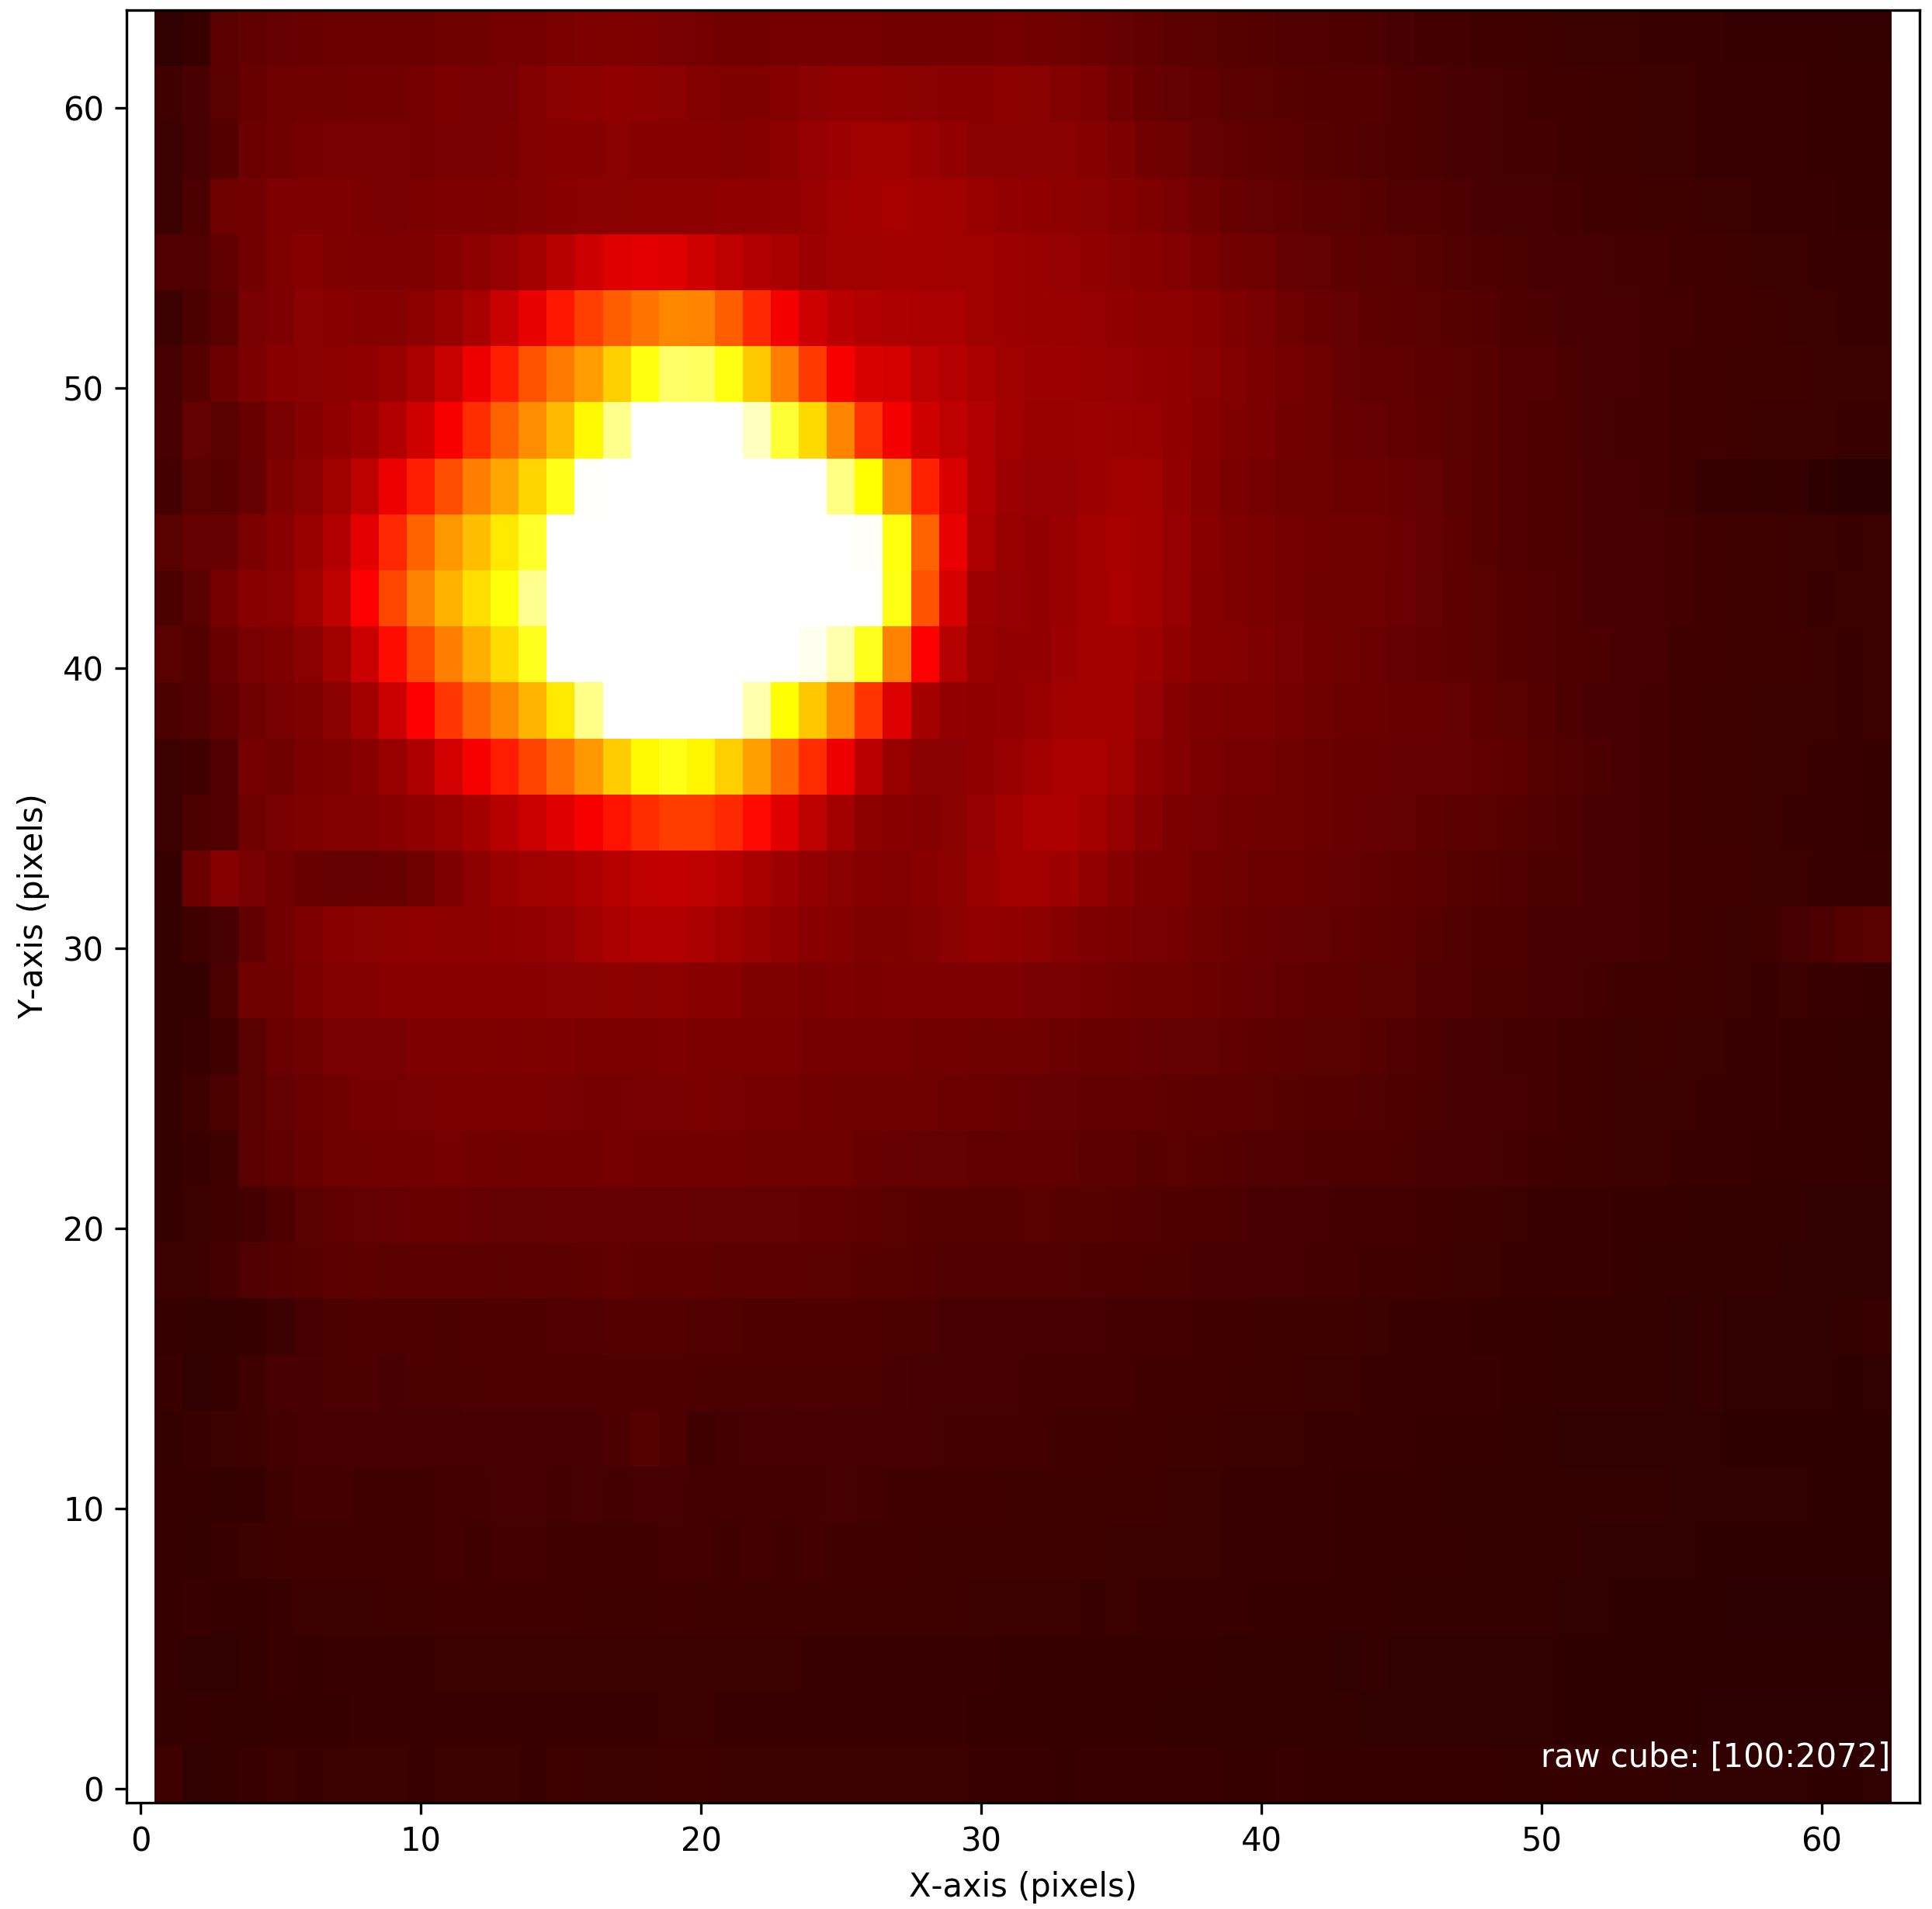
\includegraphics[width=7.8cm]{figures/SINFO_2015-02-18T07_53_Telluric_Standard_COADD_STD_H+K_0_025_full_median_collapsed_cube.png}
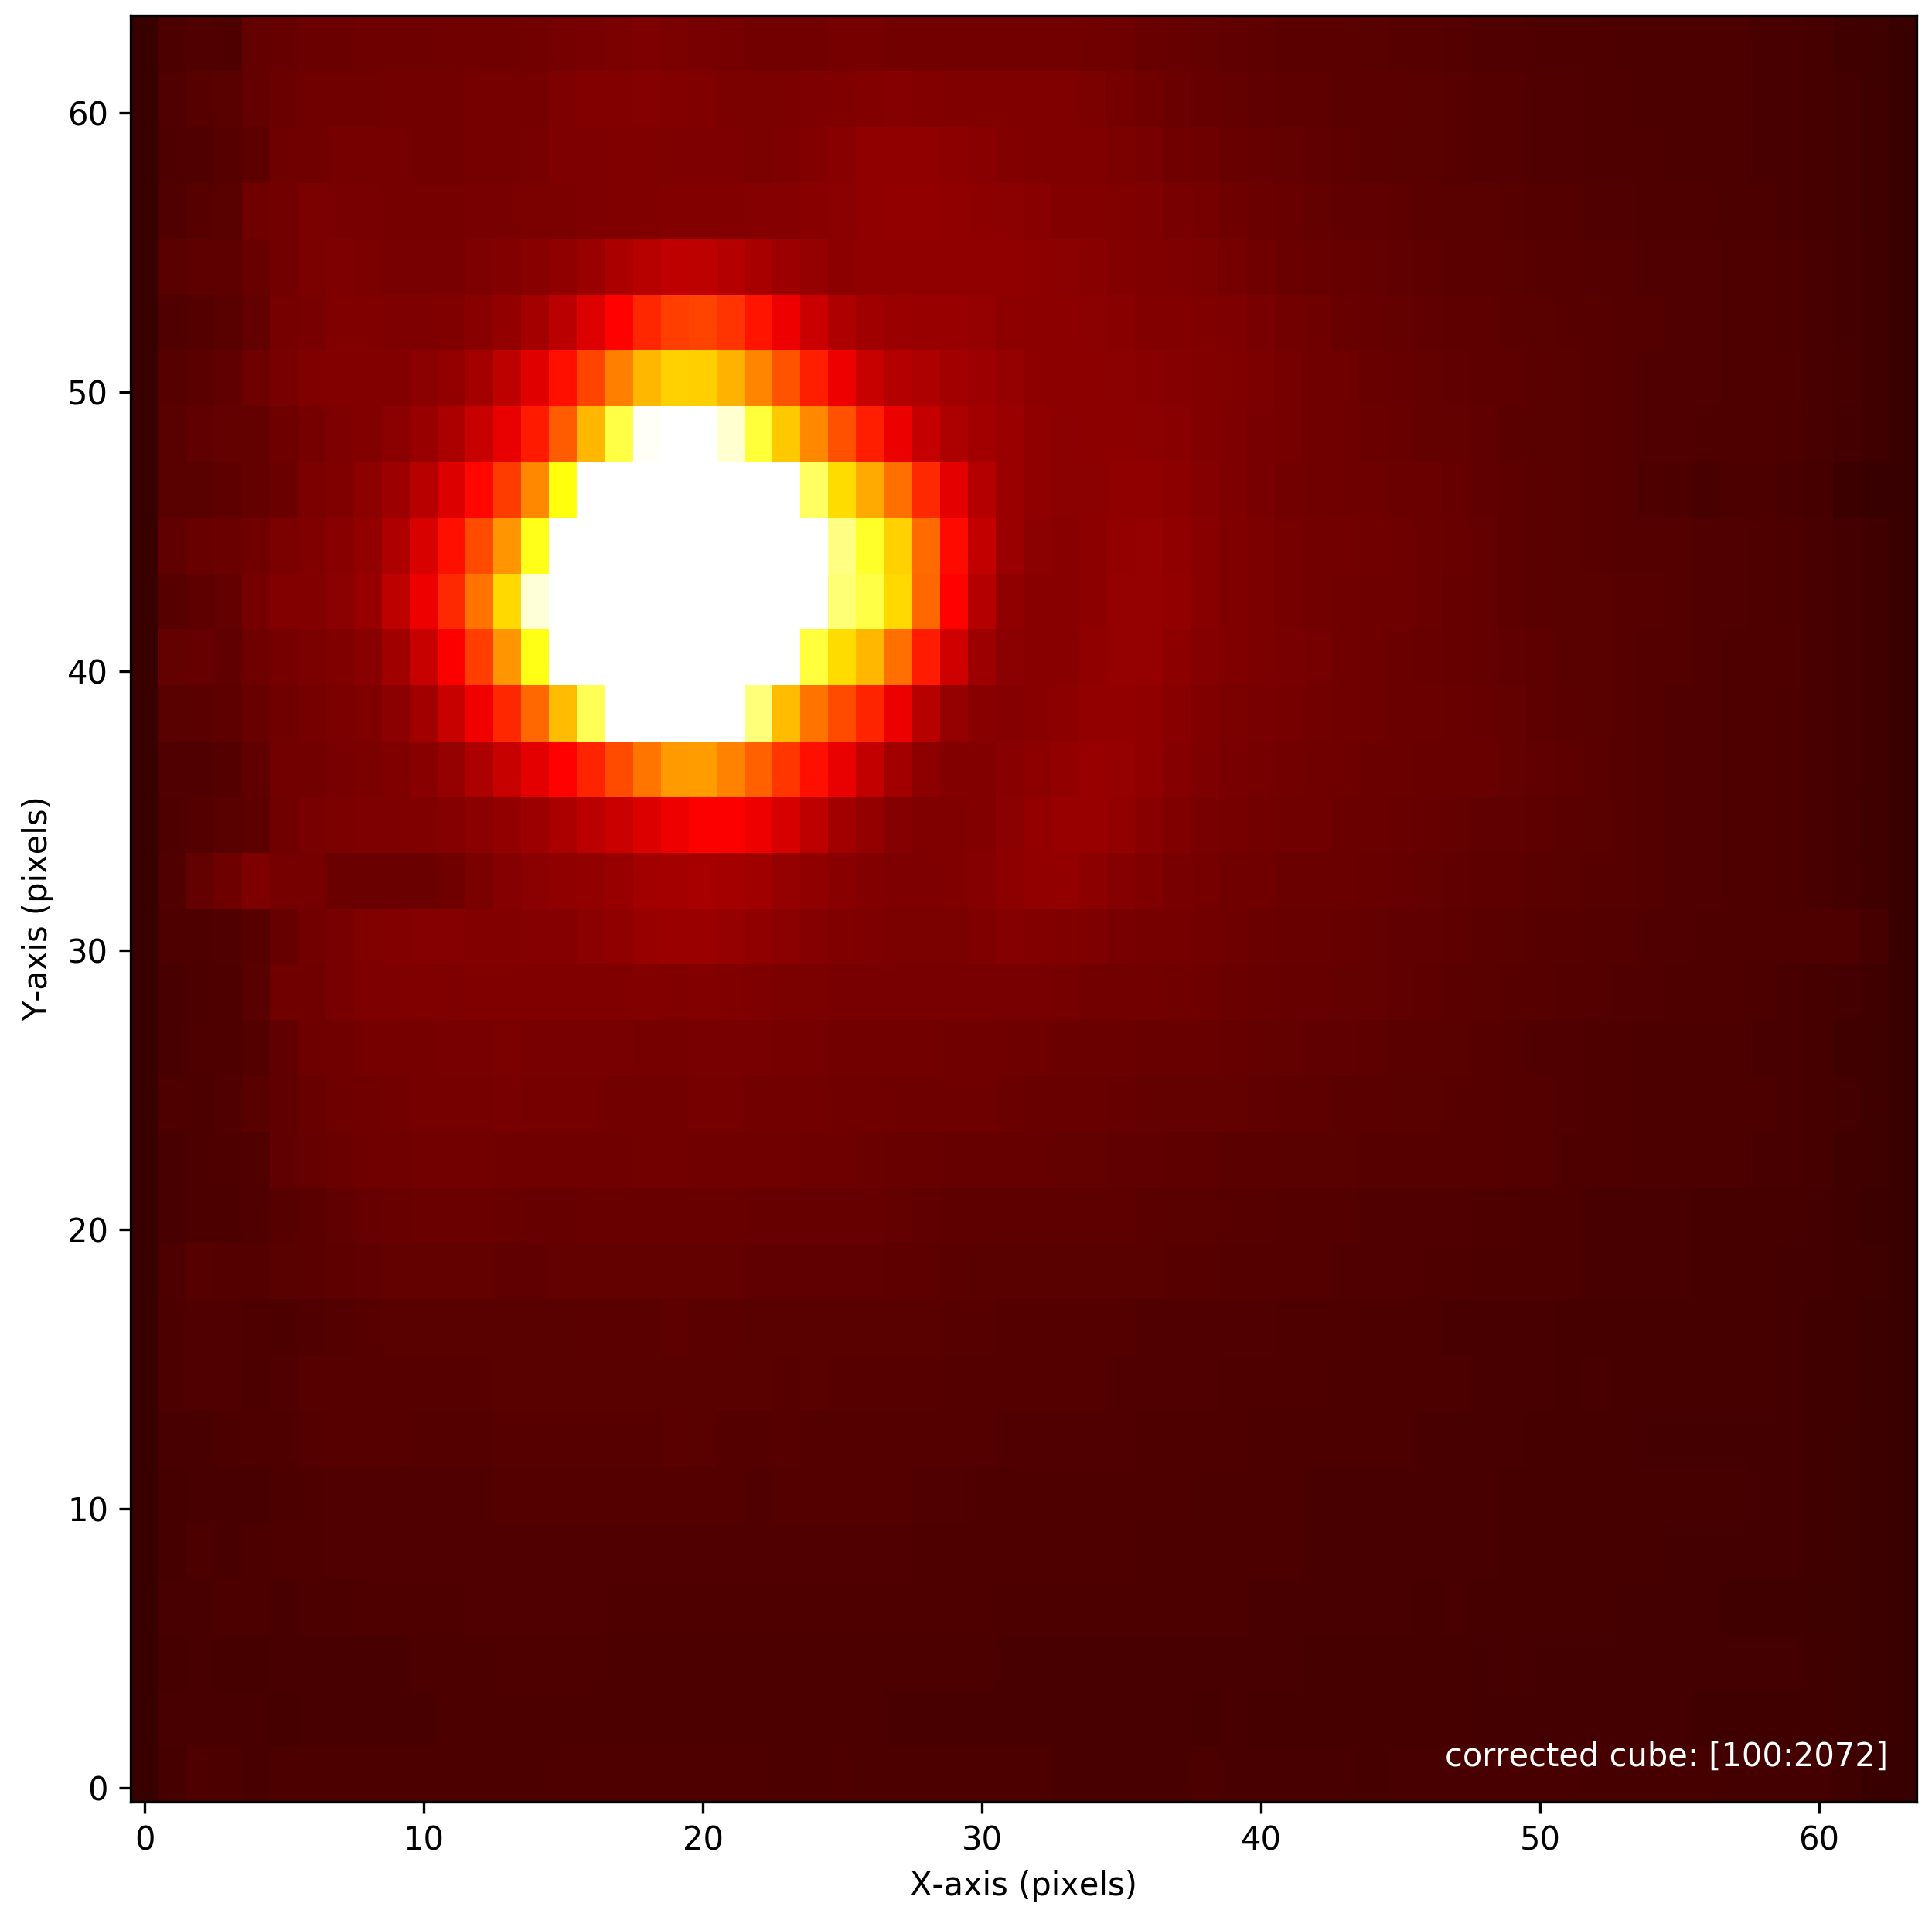
\includegraphics[width=7.8cm]{figures/SINFO_2015-02-18T07_53_Telluric_Standard_COADD_STD_H+K_0_025_full_median_corrected_cube.png}
\caption[]
	{\footnotesize  {\bf Left Panel:}  A median collapse of the same raw data cube shown as a trace in Figure \ref{fig:SINFONI_trace}. \\
	{\bf Right Panel:}  The same median collapsed cube, integer-pixel-corrected for the differential atmospheric refraction.   The improvement between the raw 
	and corrected data cubes is visually apparent.  A comparison between the raw and corrected frames reveals an x-axis FWHM of
	6.5 and 5.8 pixels, respectively.
	}
	\label{fig:SINFONI_image}
\end{figure}

\subsubsection{II.  Quantitative Results}

In order to quantify the improvements made by applying the theoretical shifts computed by \hdrldar, we define a global atmospheric refraction based the source
position at the end points of each SINFONI data cube (see Figure \ref{fig:global_offsets}).   Using the median value of the source centroid over the first 100 cube planes 
and the last 100 cube planes, we define an overall shift as: 

\begin{align}
\Delta X_c = <X_c> _{100} -  <X_c> _{N_{max} - 100}    \\
\Delta Y_c = <Y_c> _{100} -  <Y_c> _{N_{max} - 100}
\end{align}


\begin{figure}[H]
\centering \subfigure
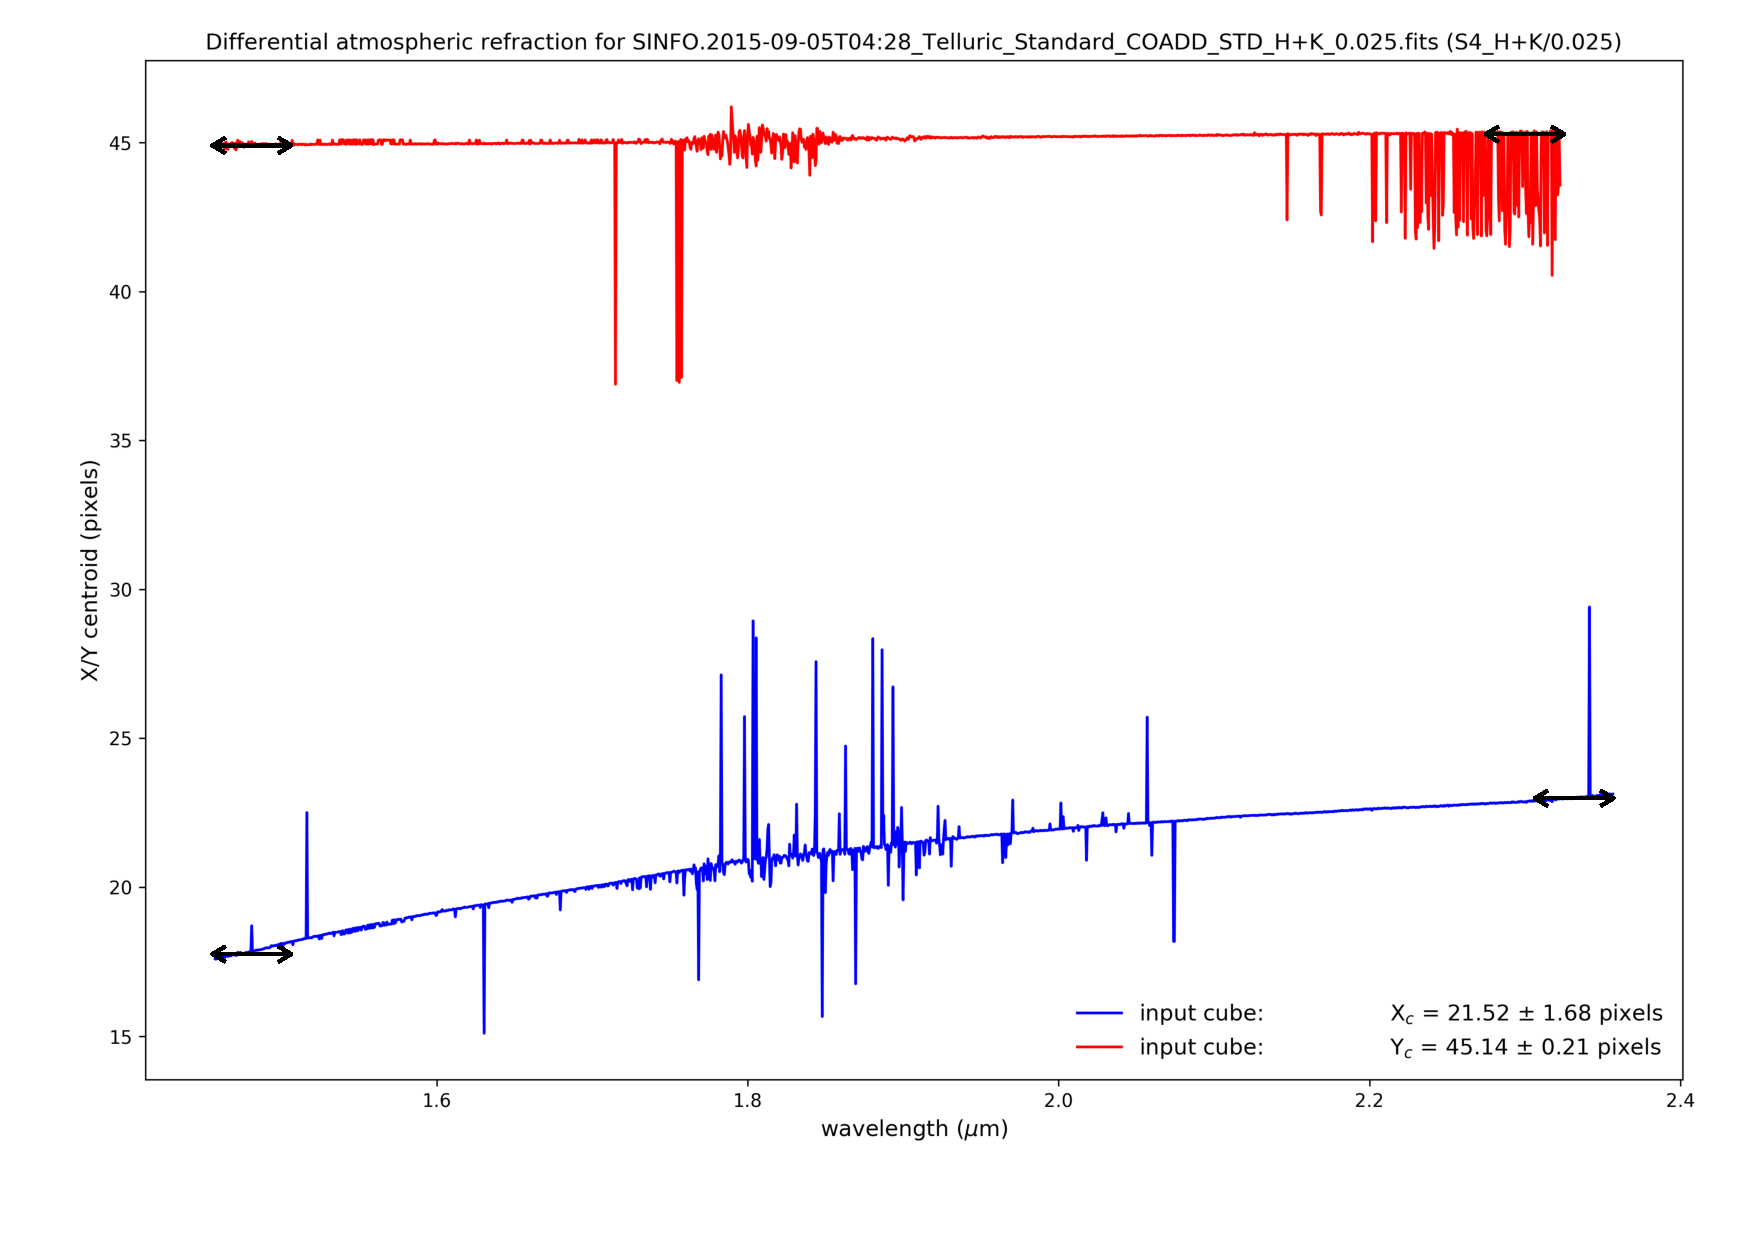
\includegraphics[width=16cm]{figures/define_global_offset.pdf} 
\caption[]
	{\footnotesize  In order to measure the global atmospheric refraction offsets in all SINFONI data cubes, the median centroid position is determined over the first
	100 and the final 100 cube planes.   This is used to define the $\Delta$X$_c$ and $\Delta$Y$_c$.
	}
	\label{fig:global_offsets}
\end{figure}


This global shift is defined for both the measured source centroids and for the theoretically predicted shifts.  For all 754 SINFONI data cubes, we find a very good
match between the measured data offsets and those predicted by \hdrldar:

\begin{align}
\Delta X_c ({\rm data}) -  \Delta X_c ({\rm theory})  = 0.29 \pm 0.63\ {\rm pixels}  \\
\Delta Y_c ({\rm data}) -  \Delta Y_c ({\rm theory})  = 0.02 \pm 0.19\ {\rm pixels}
\end{align}

It should be noted that the reconstructed SINFONI data cubes have rectangular pixels, with the Y-axis pixels being twice as large as those in the X-axis.  This
explains the difference in standard deviation measured in the offsets of equations (3) and (4). 
There appears to be a slight under-correction in the $\Delta X_c$ of about $\frac{1}{3}$ of a pixel.  However, due to the difficulty measuring the source centroids
due to object faintness and/or large background noise, this fraction of a pixel offset is not significant.

The differences between the global offsets measured in the SINFONI data cubes and the offsets predicted by \hdrldar, can be summarised in a surface density
plot displaying $\Delta X_c$(data) - $\Delta X_c$(theory) vs. $\Delta Y_c$(data) - $\Delta Y_c$(theory).   This plot is shown in Figure \ref{fig:surface_density}.


\begin{figure}[H]
\centering \subfigure
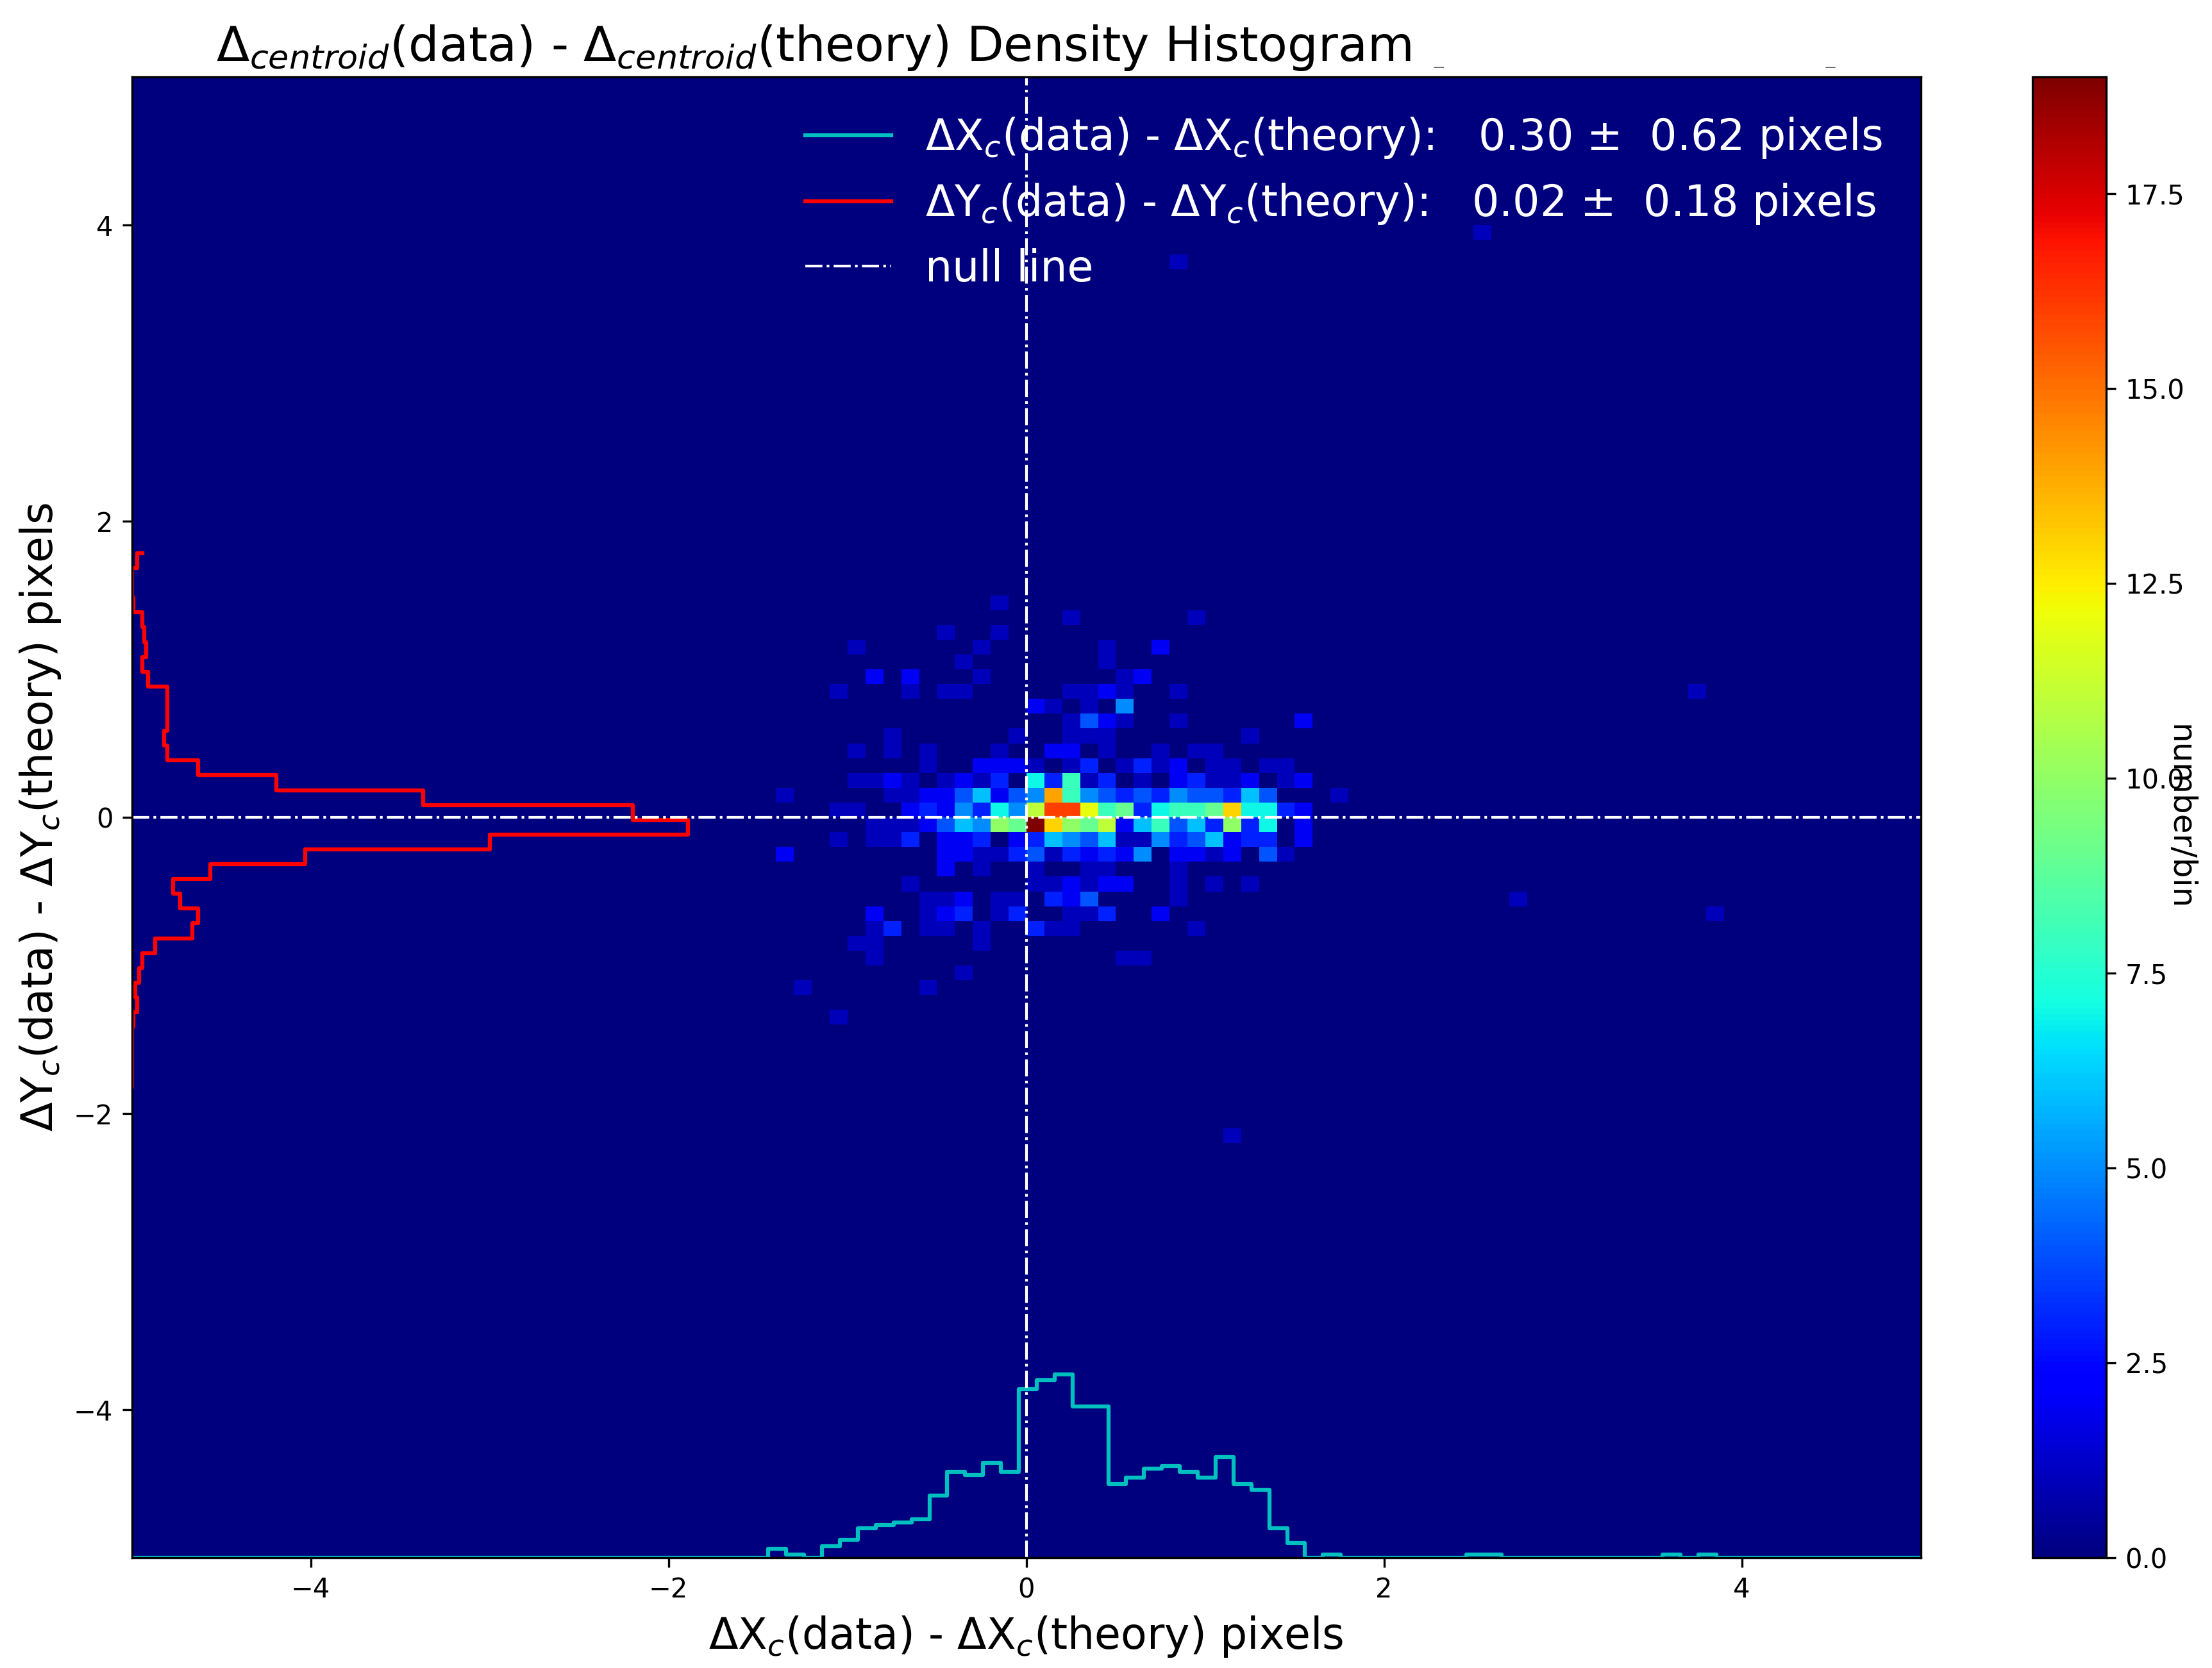
\includegraphics[width=15cm]{figures/SINFO_DAR_2014_2015_2016_surface_density.png} 
\caption[]
	{\footnotesize  Surface density plot of $\Delta X_c$(data) - $\Delta X_c$(theory) vs. $\Delta Y_c$(data) - $\Delta Y_c$(theory) for the 754 SINFONI data
	cubes analysed.  Note that the differing widths of the $\Delta X_c$ and $\Delta Y_c$ histograms is due to the fact that SINFONI has rectangular pixels
	in a 1:2 ratio for $X$:$Y$.
	}
	\label{fig:surface_density}
\end{figure}


An alternative measure of the difference between the measured and predicted offsets can be done using the residuals.  For each SINFONI data cube,
the median centroid position of the standard star was measured ($<X_c>$, $<Y_c>$).  Then, for each cube plane the shift predicted by \hdrldar\ was
added to the measured value of the source centroid and subtracted from the median centroid position.   Thus, the residuals were computed as:

\begin{align}
X_c \, {\rm residual}    =    |  <X_c ({\rm data})>  -  [X_c ({\rm data})  +  X_{\rm shift} ({\rm theory})]\  |  \hspace*{0.5cm} {\rm pixels}  \\
Y_c \, {\rm residual}    =    |  <Y_c ({\rm data})>  -  [X_c ({\rm data})  +  Y_{\rm shift} ({\rm theory})]\  |  \hspace*{0.5cm} {\rm pixels}
\end{align}

A surface density plot of these residuals are shown in Figure \ref{fig:residual_density}.  

\begin{align}
X_c \, {\rm residual}    =    0.15 \pm 0.13  \hspace*{0.5cm} {\rm pixels}  \\
Y_c \, {\rm residual}    =    0.04 \pm 0.03  \hspace*{0.5cm} {\rm pixels}
\end{align}

\begin{figure}[H]
\centering \subfigure
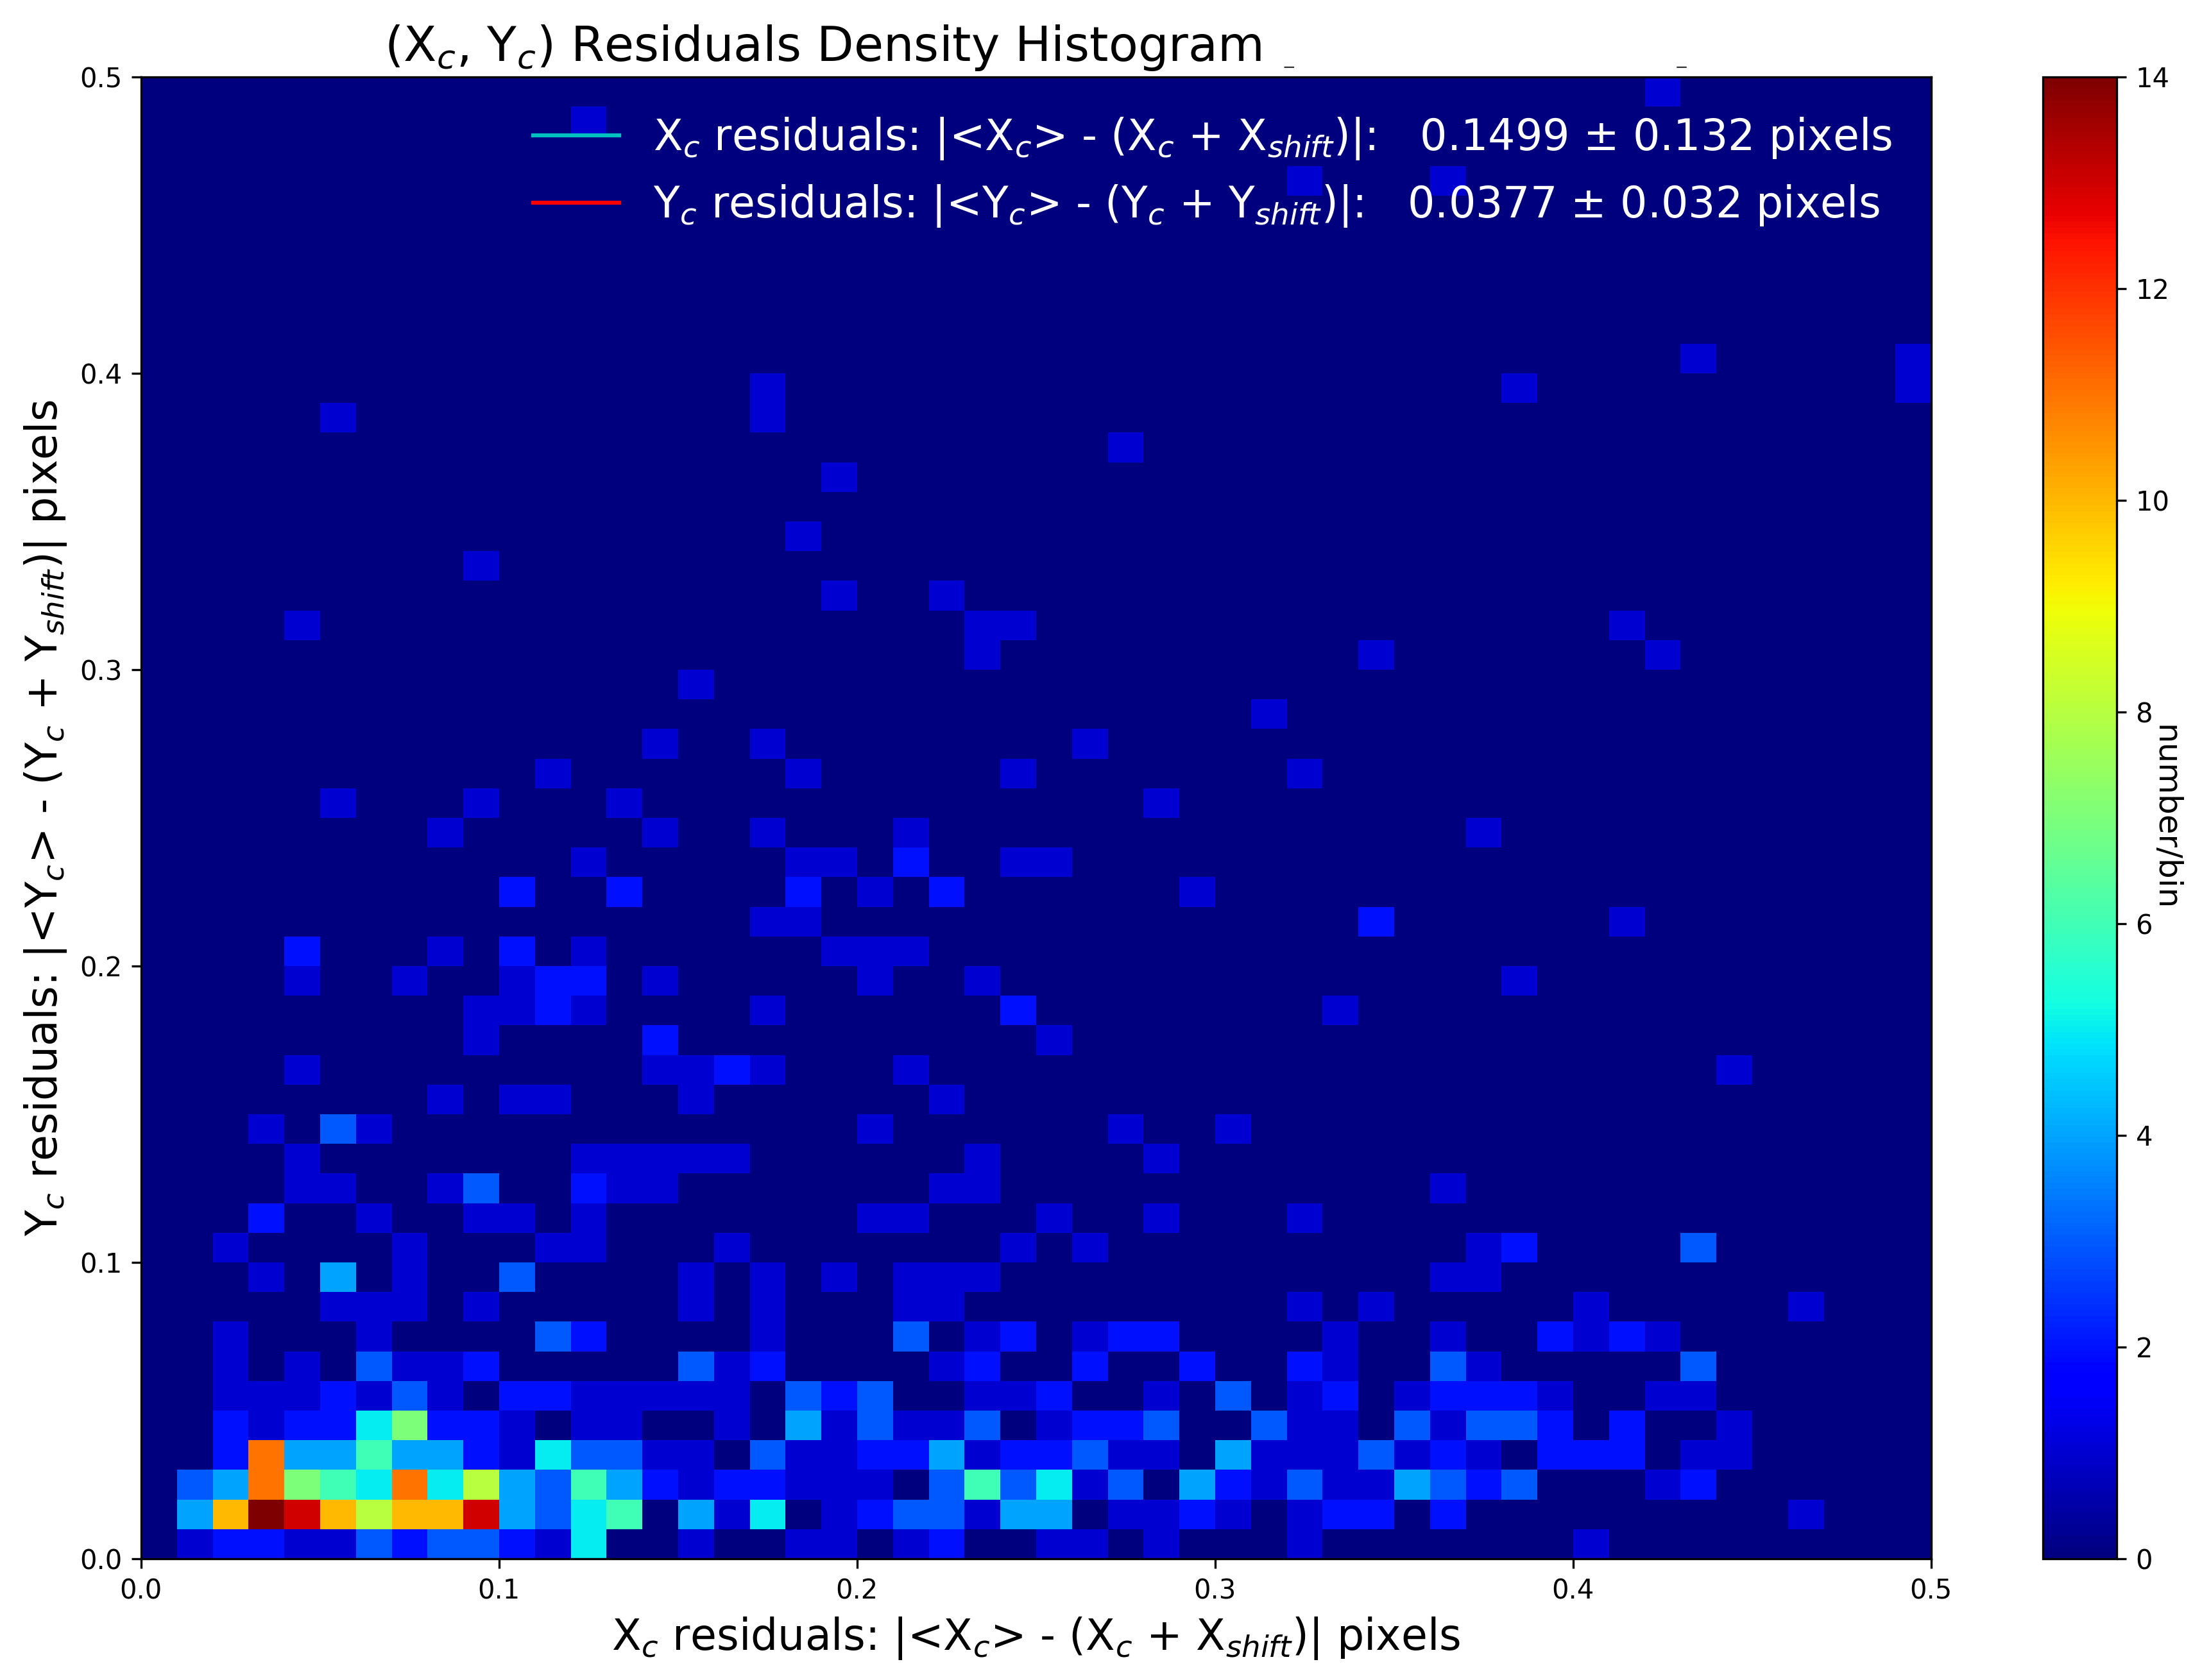
\includegraphics[width=16cm]{figures/SINFO_DAR_2014_2015_2016_residual_density.png} 
\caption[]
	{\footnotesize  Surface density residual plot of $|  <X_c ({\rm data})>  -  [X_c ({\rm data})  +  X_{\rm shift} ({\rm theory})]\  |$ vs. 
	$|  <Y_c ({\rm data})>  -  [X_c ({\rm data})  +  Y_{\rm shift} ({\rm theory})]\  |$ for the 753 SINFONI data
	cubes analysed.  Note that the differing widths of the $\Delta X_c$ and $\Delta Y_c$ histograms is due to the fact that SINFONI has rectangular pixels
	in a 1:2 ratio for $X$:$Y$.
	}
	\label{fig:residual_density}
\end{figure}

\subsubsection{The Strehl Ratios in \hdrldar-Corrected Images}

A further test was made of the improvements possible in the image quality when the \hdrldar\ correction is applied to the SINFONI standard star data cubes.
\hdrldar\ uses its calculated shifts as a function of wavelength, summarised in the results table ({\tt HDRLDEMO\_DAR\_RESULT}), to apply an integer correction 
to the source position.  This is done as the simplest correction and to avoid having to interpolate.

For each corrected data cube a median collapsed image was create and compared to the median collapsed image of the input data cube (an example of this can be
seen in Figure \ref{fig:SINFONI_image}).   For each image, {\tt SExtractor} was run using a detection and analysis threshold of 3$\sigma$.  The \hdrlstrehl\ routine
was then run on the same image using a {\tt flux-radius} set to 1.5$\times$FWHM computed by {\tt SExtractor}.   The {\tt bkg-radius-low} was set to 2.0$\times$FWHM and the
{\tt bkg-radius-high} was set to 3.0$\times$FWHM.  This analysis was restricted to the SINFONI standard star data cubes that show the largest atmospheric refraction; namely,
the $J$ and $H+K$ filters with the 25\,mas pixel scale.   The strehl ratio distributions for the 126 uncorrected (raw) and corrected data cubes are shown as histograms in 
Figure \ref{fig:strehl}.   The corrected data (green histogram) shows a marked improvement over the uncorrected data, with both the strehl median and standard deviation being 
reduced by 26\% and 32\%, respectively.  Since only an integer shift correction was made, this can be considered a lower-limit to the strehl improvement that is possible
when applying \hdrldar\ corrections.


\begin{figure}[H]
\centering \subfigure
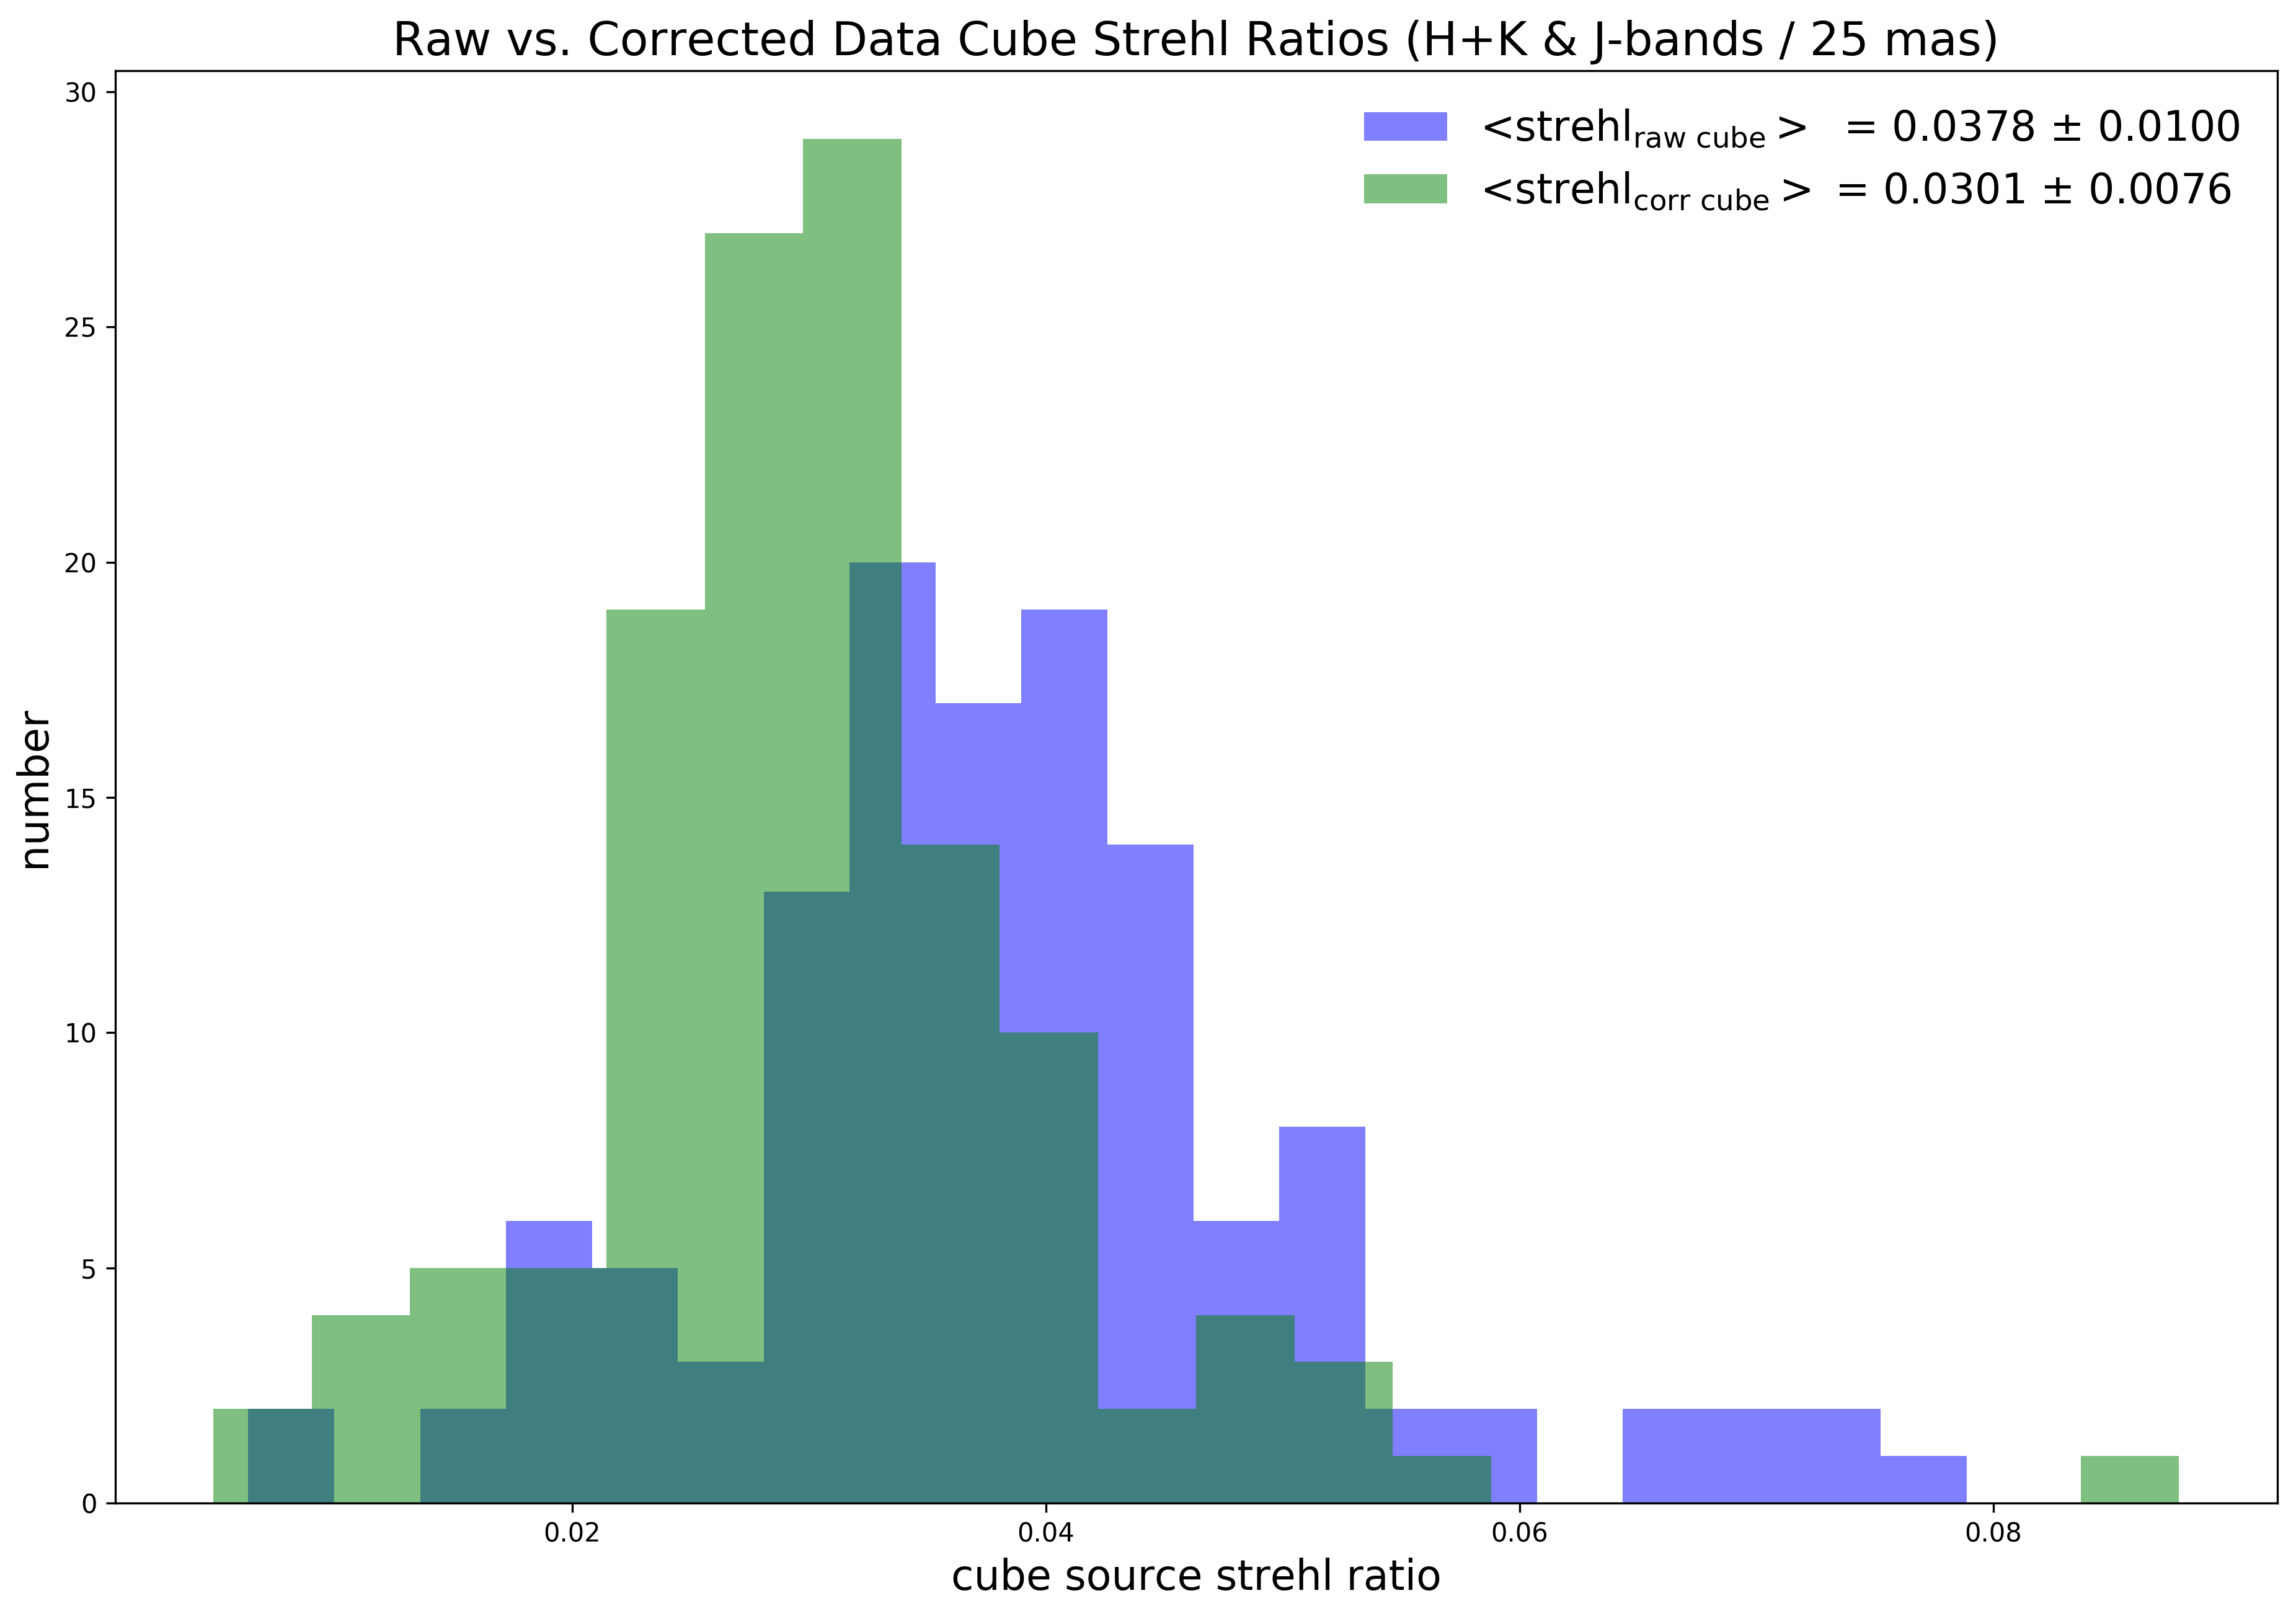
\includegraphics[width=16cm]{figures/SINFO_DAR_2014_2015_2016_HK_J_0_025_strehl20.png} 
\caption[]
	{\footnotesize  A comparison between strehl ratios measured on the median collapsed SINFONI data cubes.  The blue histogram shows the strehl ratios of the original
	data while the green histogram shows the strehl ratios of data corrected for differential atmospheric refraction using \hdrldar.  The data is restricted to the 126 SINFONI
	cubes with 25 mas pixels scale as these have the largest displacements.  The \hdrldar\ correction of the differential atmospheric refraction employed integer pixel shifts only.  
	No interpolation was done.  Despite this, the improvement is significant both in terms of the histogram distribution and in the 26\% improvement in the median strehl ratio.
	}
	\label{fig:strehl}
\end{figure}





